\chapter{植物需要什么}\label{ch:g4:what-plants-need}

两盆水芥菜摆在同一个窗台上，同一天播种。
一盆浇水，一盆不浇水——一周之内，
两者的差异便以绿色与黄色清楚地呈现出来。借助花盆、\omterm{def:g2:from-seed-to-plant:seed}{种子}与
耐心，你就能让\omterm{def:g1:plants-around-us:plant}{植物}自己回答本章的问题：
\omterm{def:g1:plants-around-us:plant}{植物}要生存和生长，究竟需要什么？

\section{向植物提问：公平试验}

\begin{method}[公平试验]\label{met:g4:what-plants-need:fairtest}
要查明\omterm{def:g1:plants-around-us:plant}{植物}是否需要某种东西——比如水、光、
土壤、温度：
\begin{enumerate}
  \item 取\emph{两}盆同种\omterm{def:g1:plants-around-us:plant}{植物}，
        播种方式相同；
  \item 除\emph{被检验的那一项}外，其余一切完全相同
——一盆给予该条件，另一盆不给予；
  \item 等待数日或数周，然后比较；
  \item 若两盆之间有任何差异，必定来自你所改变的那一项：
        这次试验便是公平的。
\end{enumerate}
未做处理的花盆称为\emph{对照}\index{对照（实验）}：它显示的是一切条件都不缺失时的结果。
\end{method}

\begin{example}[为什么用两盆而不用一盆]\label{ex:g4:what-plants-need:control}
假设一盆未浇水的花盆枯萎了。是缺水的缘故，
还是寒流，或是\omterm{def:g2:from-seed-to-plant:seed}{种子}不好？若身旁有一盆浇了水的“孪生”花盆，
与它来自同一包\omterm{def:g2:from-seed-to-plant:seed}{种子}、置于同一房间，依然青翠，
两者的差异仅在于水，疑虑便消失了。
只用一盆做的试验，没有人会相信，生物学家尤其不会。
\end{example}


\begin{omfigure}
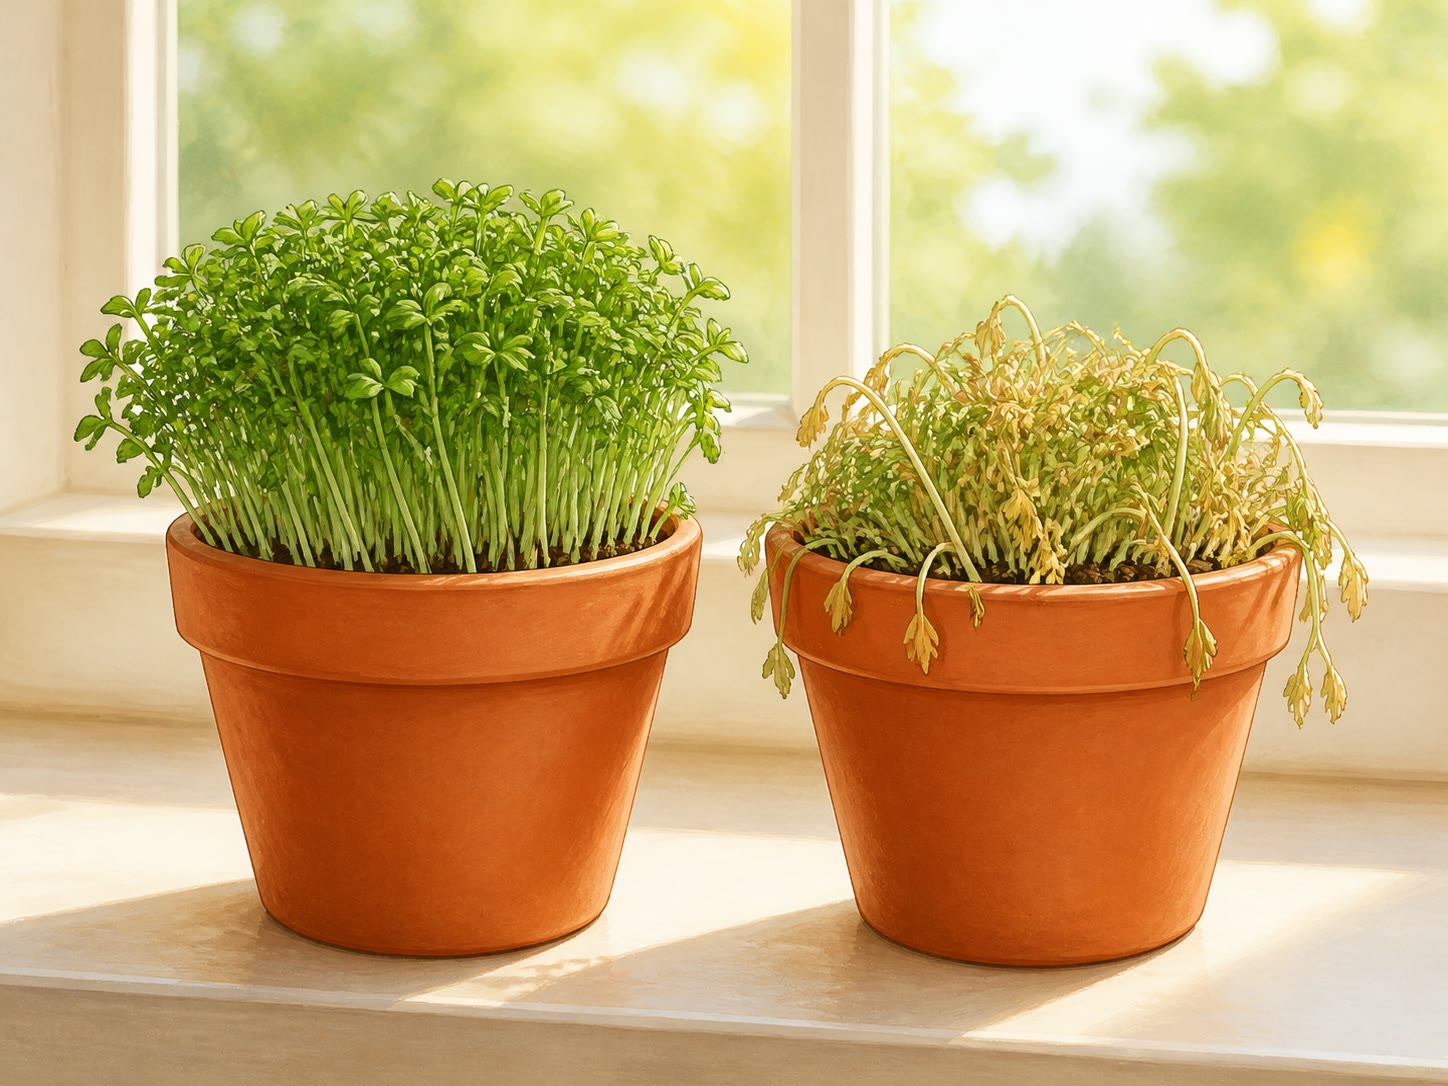
\includegraphics[width=0.58\linewidth]{images/book1/ai/g4-plants-cresspots.jpg}

{\small 同一实验在真实窗台上进行，一周后：
两盆\omterm{def:g1:plants-around-us:plant}{植物}现在在所有可见方面都不同——因为
它们只在一件事上存在差别。}
\end{omfigure}

\section{试验揭示了什么}

\begin{proposition}[植物的需要]\label{prop:g4:what-plants-need:needs}
逐一对每种需要进行公平试验，结果表明\omterm{def:g1:plants-around-us:plant}{植物}需要：
\begin{itemize}
  \item \emph{水}——未浇水的花盆枯萎死亡；
  \item \emph{光}——放在柜子里的花盆生长得苍白、细长而
        虚弱，最后便不再生长：没有光，就无法制造养分；
  \item \emph{空气}——与新鲜空气隔绝，生长停止；
  \item \emph{温度}——在寒冷中，\omterm{def:g2:from-seed-to-plant:seed}{种子}静静等待
        （见\cref{prop:g2:from-seed-to-plant:needs}），生长
        随之凝固停止；
  \item \emph{无机盐}\index{无机盐}：极少量的营养物质，
        根从土壤中吸收，它们溶解在土壤水分里，
        仅有纯水时，\omterm{def:g1:plants-around-us:plant}{植物}
        很快就会缺乏。
\end{itemize}
\end{proposition}
\admitted

\begin{example}[苍白的“囚徒”]\label{ex:g4:what-plants-need:pale}
\cref{exo:g1:plants-around-us:8}中的柜子试验，
若认真地与一盆受光的“孪生”\omterm{def:g1:plants-around-us:plant}{植物}一同进行，会得到醒目的结果：囚徒
不仅萎靡，而且\emph{淡黄色}——它停止了制造
叶绿素——并且奇怪地\emph{变高}，身子伸得长长的，
仿佛在寻找缺失的光。没有光的生长，就像
只有支出没有收入；\omterm{def:g2:from-seed-to-plant:seed}{种子}的储备一旦耗尽，它
便停止了生长。
\end{example}

\begin{remark}[园丁为什么要给土壤施肥]\label{rem:g4:what-plants-need:soil}
堆肥和粪肥并不是\omterm{def:g1:plants-around-us:plant}{植物}的“餐食”——\omterm{def:g1:plants-around-us:plant}{植物}
不吃任何\omterm{def:g1:living-or-not:living}{生物}。它们补充土壤中的\omterm{prop:g4:what-plants-need:needs}{无机盐}，
这些\omterm{prop:g4:what-plants-need:needs}{无机盐}会随着收获年复一年地被带走。
\cref{ex:g2:caring-for-nature:compost}中的堆肥箱构成一个闭环：
土壤供给蔬菜的物质，经由菜皮与果皮又回到土壤中。
\end{remark}

\section{植物如何利用所吸收的物质}

\begin{proposition}[植物自行制造物质]\label{prop:g4:what-plants-need:make}
\omterm{def:g1:animals-around-us:animal}{动物}通过吃其他\omterm{def:g1:living-or-not:living}{生物}而生长。\omterm{def:g1:plants-around-us:plant}{植物}不吃任何\omterm{def:g1:living-or-not:living}{生物}：
它借助土壤中的水和\omterm{prop:g4:what-plants-need:needs}{无机盐}、空气，以及
绿叶捕获的\emph{光}所带来的\omterm{prop:g3:balanced-diet:jobs}{能量}，它
\emph{制造自身的物质}——新的茎、叶、根和\omterm{def:g2:from-seed-to-plant:seed}{种子}。这就是为什么
光对\omterm{def:g1:plants-around-us:plant}{植物}来说和食物、饮水一样重要，这也是为什么绿叶
总是朝向天空。
\end{proposition}
\admitted

\begin{example}[几乎凭空长出的一棵树]\label{ex:g4:what-plants-need:tree}
在一只大花盆里种下一粒\omterm{def:g2:from-seed-to-plant:seed}{种子}，土壤已事先称过重量，等上数年，
便会有一棵小树立在那里——然而土壤几乎没有减轻
分量。树的木材并非从花盆里挖出：它是
\emph{制造}出来的，由水、空气和光，在叶片这座
绿色工坊里制成。\omterm{def:g1:living-or-not:living}{生物}体的物质从何而来，
这个问题我们在以后的学习中还会再探讨。
\end{example}

\begin{remark}[绿色供养每一个人]\label{rem:g4:what-plants-need:everyone}
回想\cref{prop:g3:food-chains:start}：每一条\omterm{def:g3:food-chains:chain}{食物链}都始于
一种\omterm{def:g1:plants-around-us:plant}{植物}。现在我们明白了这为何必然如此——\omterm{def:g1:plants-around-us:plant}{植物}是
唯一能用\omterm{def:g1:living-or-not:nonliving}{非生物}原料制造新物质的环节。
无论何处，每个人吃下的每一口食物，都先在叶片中制成。
\end{remark}

\section{练习}

\begin{exercise}[$\star$]\label{exo:g4:what-plants-need:1}
列出\omterm{def:g1:plants-around-us:plant}{植物}的五种需要。
\end{exercise}

\begin{exercise}[$\star$]\label{exo:g4:what-plants-need:2}
在公平检验中，两个
花盆之间可能有几样东西不同？那个未做处理的花盆称为什么？
\end{exercise}

\begin{exercise}[$\star$]\label{exo:g4:what-plants-need:3}
描述在黑暗中培养了两周的
\omterm{def:g1:plants-around-us:plant}{植物}的外观。缺少的是哪一种需要？它无法制造什么？
\end{exercise}

\begin{exercise}[$\star$]\label{exo:g4:what-plants-need:4}
什么是\omterm{prop:g4:what-plants-need:needs}{无机盐}？\omterm{def:g1:plants-around-us:plant}{植物}是如何吸收的？
\end{exercise}

\begin{exercise}[$\star$]\label{exo:g4:what-plants-need:5}
为什么园丁要施用堆肥，既然\omterm{def:g1:plants-around-us:plant}{植物}并不进食？
\end{exercise}

\begin{exercise}[$\star$]\label{exo:g4:what-plants-need:6}
\omterm{def:g1:plants-around-us:plant}{植物}的生长方式与\omterm{def:g1:animals-around-us:animal}{动物}有何不同，
依据\cref{prop:g4:what-plants-need:make}？
\end{exercise}

\begin{exercise}[$\star$]\label{exo:g4:what-plants-need:7}
在\cref{ex:g4:what-plants-need:tree}中，花盆里的土壤在树生长时几乎
没有减少重量。树的物质
来自何处？
\end{exercise}

\begin{exercise}[$\star$]\label{exo:g4:what-plants-need:8}
动手试一试：设计并进行图中的水分公平检验，用水芥菜
做材料——两个花盆，只有一处不同。记录
一周后你所看到的现象。
\end{exercise}

\begin{exercise}[$\star\star$]\label{exo:g4:what-plants-need:9}
卢卡斯“证明”\omterm{def:g1:plants-around-us:plant}{植物}需要音乐：他对一个花盆唱歌，
唱了一个月，这盆\omterm{def:g1:plants-around-us:plant}{植物}长势良好。他的实验缺少了什么，
依据\cref{met:g4:what-plants-need:fairtest}？请设计一个
真正能检验这一点的版本。
\end{exercise}

\begin{exercise}[$\star\star$]\label{exo:g4:what-plants-need:10}
一种水生\omterm{def:g1:plants-around-us:plant}{植物}完全浸没在水中生长，没有根，却十分健康。
它显然仍在满足五种需要中的哪一种？它是如何满足的，
——哪一种需要由水分供应代替了土壤所起的作用？
\end{exercise}

\begin{exercise}[$\star\star\star$]\label{exo:g4:what-plants-need:11}
两盆一模一样的薄荷：一盆种在只浇灌纯净雨水的沙子里，一盆种在
花园土壤里，两盆都以同样的方式浇水、光照。两个月后，
沙子里的那盆植株变得矮小、\omterm{def:g1:plants-around-us:parts}{叶子}发黄。这一公平检验
隔离出的是哪一种需要？为何沙子里的植株起初仍能生长？
\end{exercise}
